\documentclass[a4paper]{article}

\usepackage[margin=1in]{geometry}
\usepackage{amsmath}
\usepackage{amssymb}
\usepackage{graphicx}
\usepackage{float}
\usepackage{hyperref}
\usepackage{caption}
\usepackage{subcaption}
\usepackage{amsfonts}
\usepackage{pdfpages}
\usepackage[justification=centering]{caption}

\def\sectionautorefname{Section}
\def\subsectionautorefname{Section}
\def\subsubsectionautorefname{Section}
\def\figureautorefname{Figure}
\def\tableautorefname{Table}
\def\equationautorefname{Equation}


\begin{document}

%%%%%%%%%%%%%%%%%%%%%%%%%%
%%%%%%%%%%%%%%%%%%%%%%%%%%

\title{Random number generation}
\author{3F3 laboratory experiment: Full Technical Report \\ Theo A. Brown \\ Selwyn College, University of Cambridge}
\date{\today}
\maketitle

\tableofcontents
\newpage

%%%%%%%%%%%%%%%%%%%%%%%%%%
%%%%%%%%%%%%%%%%%%%%%%%%%%

\section{Introduction}
Random numbers are widely used in science and engineering, forming the basis of stochastic modelling and inference.
Generators of Gaussian and Uniform random numbers are widely implemented, but in many applications samples from more
complex distributions are required.
This report investigates methods for generating random numbers from different distributions.
Firstly, Uniform and Gaussian random number generators are used to investigate different methods for estimating
probability density functions (PDFs) from samples.
Secondly, samples from a new distribution are generated by transforming samples from a Uniform or Gaussian distribution,
using the Jacobian of the transformation.
Thirdly, Uniformly distributed random samples are transformed using the inverse cumulative density function of the
desired distribution.
Finally, samples from very complex distributions are generated using a scaled mixture of Gaussians, where the desired
distribution can be written as a Gaussian distribution with a random variance, set by some PDF.
In addition, Monte Carlo methods for estimating properties of a distribution from samples are investigated.


%%%%%%%%%%%%%%%%%%%%%%%%%%
%%%%%%%%%%%%%%%%%%%%%%%%%%

\section{Generating random numbers from the Uniform and Normal distributions}
\label{sec:uniform_normal}

A vector of 10000 samples from a unit Gaussian distribution was generated using \verb`np.random.randn`, and a vector of
10000 samples from a unit Uniform distribution was generated using \verb`np.random.rand`.
These sample vectors are used throughout the experiment to investigate different methods of random number generation.

%%%%%%%%%%%%%%%%%%%%%%%%%%

\subsection{Comparison of histogram with true probability density function}

The sample vectors were binned and plotted as histograms.
The true analytical probability density function (PDF) was calculated for the unit Gaussian and unit Uniform
distributions, and was overlaid on the histogram plots (\autoref{fig:histogram_and_pdf}).
It can be seen in \autoref{fig:histogram_and_pdf} that the histograms closely follow the shape of the analytical PDF,
showing that the generation of the random numbers for these distributions is accurate, and that histograms provide a
good method for approximating the true PDF.

\begin{figure}[h]
    \centering
    \begin{subfigure}[b]{0.45\textwidth}
        \centering
        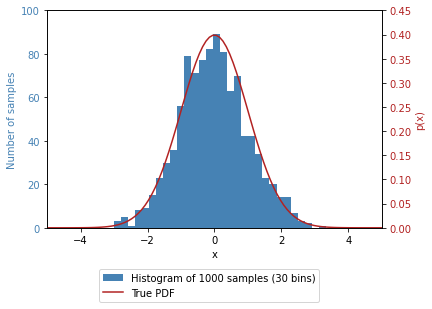
\includegraphics[width=\textwidth]{figures/gaussian_histogram_and_pdf.png}
        \caption{Gaussian distribution}
        \label{fig:gaussian_histogram_and_pdf}
    \end{subfigure}
    \hfill
    \begin{subfigure}[b]{0.45\textwidth}
        \centering
        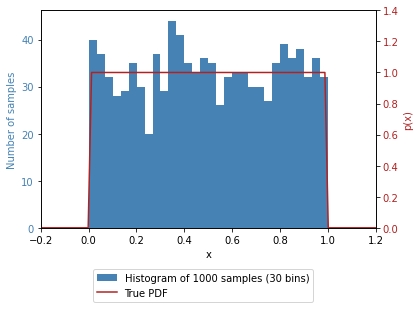
\includegraphics[width=\textwidth]{figures/uniform_histogram_and_pdf.png}
        \caption{Uniform distribution}
        \label{fig:uniform_histogram_and_pdf}
    \end{subfigure}
    \caption{Histogram of samples drawn from a distribution, overlaid with the true PDF of the distribution}
    \label{fig:histogram_and_pdf}
\end{figure}

%%%%%%%%%%%%%%%%%%%%%%%%%%

\subsection{Kernel density smoothing}

A unit Gaussian kernel $\mathcal{N}(0, 1)$ is applied to the data to provide a continuous estimate for the PDF.
The result is plotted for the Gaussian and Uniform distributions in \autoref{fig:kernel_smoothed}.

\begin{figure}[h]
    \centering
    \begin{subfigure}[b]{0.45\textwidth}
        \centering
        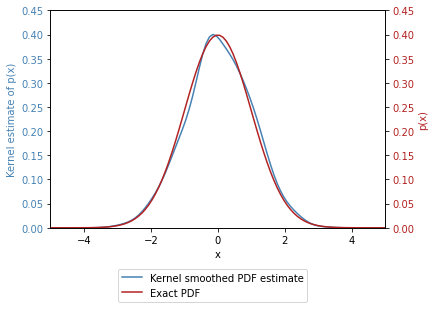
\includegraphics[width=\textwidth]{figures/gaussian_kernel_smoothed.png}
        \caption{Gaussian distribution}
        \label{fig:gaussian_kernel_smoothed}
    \end{subfigure}
    \hfill
    \begin{subfigure}[b]{0.45\textwidth}
        \centering
        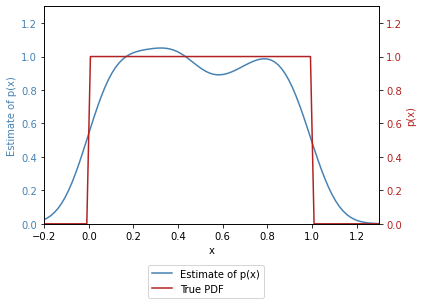
\includegraphics[width=\textwidth]{figures/uniform_kernel_smoothed.png}
        \caption{Uniform distribution}
        \label{fig:uniform_kernel_smoothed}
    \end{subfigure}
    \caption{Estimate of the PDF of a distribution, generated using Gaussian kernel smoothing of random samples from the
             distribution, overlaid with the true PDF of the distribution}
    \label{fig:kernel_smoothed}
\end{figure}

At each point, the kernel method takes the mean of N neighbouring values, weighted using a Gaussian distribution.
This is advantageous as it can smooth random irregularities in the samples: for example, there may be histogram bins
with a sample count that is greater than the expected sample count, which would give an incorrectly high estimate of
the probability of a sample falling in this bin; the kernel smooths out this local peak by taking neighbouring values
into account.
However, this also means that the kernel smoothing method becomes inaccurate when there is a sudden change or
discontinuity in the probability density function.
In the Uniform distribution there is zero probability for values outside the range $0<x<1$, but as the kernel averages
over a window of values it does not capture the step change at $x=0$ and $x=1$ and instead decays smoothly.

%%%%%%%%%%%%%%%%%%%%%%%%%%

\subsection{Multinomial distribution theory}

Multinomial distribution theory can be used to find properties of a distribution from a histogram of samples.

\subsubsection{Derivation of the multinomial distribution}
For $N$ samples and $M$ bins, let $N_i$ be the random variable representing the number of samples in bin $i$ and $p_i$
be the probability that a sample falls in bin $i$.
Samples are drawn independently, so the probability of getting $n_i$ samples in bin $i$ is given by:
\begin{align*}
    Pr(N_i = n_i) = \prod_{j=1}^{n_i} p_i = p_i^{n_i}
\end{align*}
The joint probability of obtaining a given distribution of $N$ samples across $M$ bins is given by:
\begin{align}
    \label{eq:joint_bin_probability_1}
    Pr(N_1 = n_1, N_2 = n_2, \dots, N_M= n_M) =
     \prod_{i=1}^{M} {N_{\text{available}, i} \choose {n_i}} p_i^{n_i}
\end{align}
where $N_{\text{available}, i} = N - \sum_{j=1}^{i-1} n_j$.

The binomial coefficient in \autoref{eq:joint_bin_probability_1} comes from considering all possible combinations of
getting $n_i$ samples in bin $i$:
\begin{itemize}
    \item For the first bin, $n_1$ samples are chosen from a set of $N$
    \item For the second bin, $n_2$ samples are chosen from a set of $N - n_1$
    \item For the $i$th bin, $n_i$ samples are chosen from a set of $N - n_1 \dots - n_{i-1}$
\end{itemize}
Simplifying the coefficient in \autoref{eq:joint_bin_probability_1} gives:
\begin{align*}
    {N \choose n_1}{N - n_1 \choose n_2} \dots {n_M \choose n_M}
  & = \frac{N!}{n_1!(N - n_1)!} \frac{(N - n_1)!}{n_2!(N - n_1 - n_2)!} \dots \frac{n_M!}{n_M!} \\
  & = \frac{N!}{n_1! n_2! \dots n_M!}
\end{align*}
The last step above is obtained by diagonal cancellation.

Consequently, \autoref{eq:joint_bin_probability_1} simplifies to:
\begin{align*}
    Pr(N_1 = n_1, N_2 = n_2, \dots, N_M = n_M) = \frac{N!}{n_1! n_2! \dots n_M!} p_1^{n_1} p_2^{n_2} ... p_M^{n_M}
\end{align*}

From considering the probability $p_i = Pr(N_i = n_i)$ for $N$ samples, the mean and standard deviation of $N_i$ can be
found:
\begin{align}
    \label{eq:bin_mean}
    \mu_i &= \mathbb{E}[N_i] = N p_i \\
    \label{eq:bin_sd}
    \sigma_i &= \sqrt{Var[N_i]} = \sqrt{N p_i (1 - p_i)}
\end{align}

%%%%%%%%%%%%%%%%%%%%%%%%%%

\subsubsection{Application to the Uniform distribution}
For the Uniform distribution between 0 and 1, the pdf $p(x)$ is defined as:
\begin{align*}
    p(x) &= \frac{1}{x_{max} - x_{min}} \\
         &= 1
\end{align*}
Hence, using \autoref{eq:bin_mean} and \autoref{eq:bin_sd}, the mean and standard deviation of the number of samples
from the Uniform distribution in a histogram with bin width $\delta$ and bin centers $c_i$ can be calculated:
\begin{align*}
    p_i &= \int_{c_i - \frac{\delta}{2}}^{c_i + \frac{\delta}{2}}1\,dx \\
        &= \delta \\
    \mu_i &= N \delta \\
    \sigma_i &= \sqrt{N \delta (1 - \delta)}
\end{align*}

\begin{figure}[h]
    \centering
    \begin{subfigure}[b]{0.3\textwidth}
        \centering
        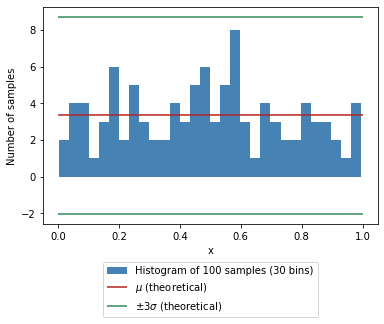
\includegraphics[width=\textwidth]{figures/uniform_histogram_100.png}
        \caption{$N=100$}
        \label{fig:uniform_histogram_100}
    \end{subfigure}
    \hfill
    \begin{subfigure}[b]{0.3\textwidth}
        \centering
        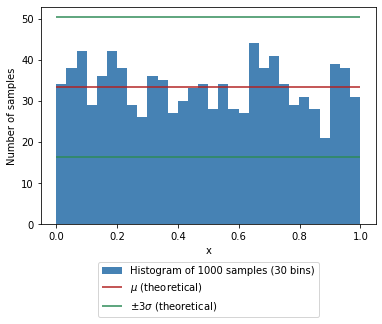
\includegraphics[width=\textwidth]{figures/uniform_histogram_1000.png}
        \caption{$N=1000$}
        \label{fig:uniform_histogram_1000}
    \end{subfigure}
    \hfill
    \begin{subfigure}[b]{0.3\textwidth}
        \centering
        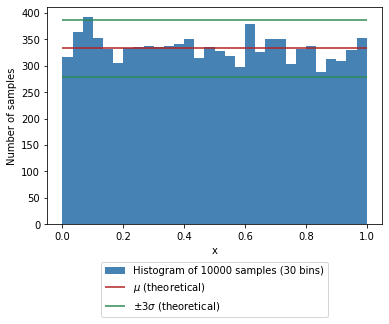
\includegraphics[width=\textwidth]{figures/uniform_histogram_10000.png}
        \caption{$N=10000$}
        \label{fig:uniform_histogram_10000}
    \end{subfigure}
    \caption{Histogram of N samples from a Uniform distribution, showing mean and $\pm3$ standard deviation}
    \label{fig:uniform_histogram_increasing_N}
\end{figure}

\autoref{fig:uniform_histogram_increasing_N} shows that the sample count lies within the $3\sigma$ interval for almost
all bins, which is consistent with the multinomial distribution theory.

%%%%%%%%%%%%%%%%%%%%%%%%%%

\subsubsection{Application to the Gaussian distribution}

For the Gaussian distribution:
\begin{align*}
        p_i &= \int_{c_i - \frac{\delta}{2}}^{c_i + \frac{\delta}{2}} \frac{1}{\sqrt{2 \pi \sigma}} \exp \left(-\frac{1}{2} x^2 \right) \,dx \\
        &= \Phi \left(c_i + \frac{\delta}{2}\right)- \Phi\left(c_i - \frac{\delta}{2}\right)
\end{align*}

The mean and variance for each bin are calculated according to \autoref{eq:bin_mean} and \autoref{eq:bin_mean}.

\begin{figure}[h]
    \centering
    \begin{subfigure}[b]{0.3\textwidth}
        \centering
        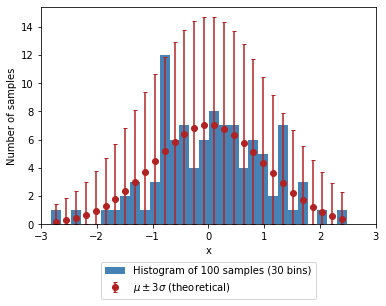
\includegraphics[width=\textwidth]{figures/gaussian_histogram_100.png}
        \caption{$N=100$}
        \label{fig:gaussian_histogram_100}
    \end{subfigure}
    \hfill
    \begin{subfigure}[b]{0.3\textwidth}
        \centering
        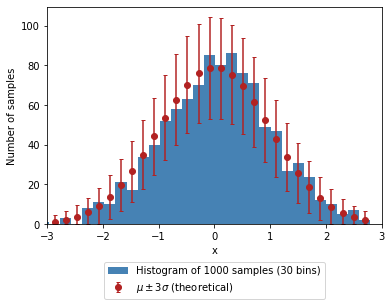
\includegraphics[width=\textwidth]{figures/gaussian_histogram_1000.png}
        \caption{$N=1000$}
        \label{fig:gaussian_histogram_1000}
    \end{subfigure}
    \hfill
    \begin{subfigure}[b]{0.3\textwidth}
        \centering
        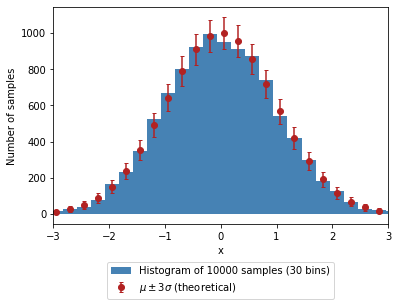
\includegraphics[width=\textwidth]{figures/gaussian_histogram_10000.png}
        \caption{$N=10000$}
        \label{fig:gaussian_histogram_10000}
    \end{subfigure}
    \caption{Histogram of N samples from a Gaussian distribution, showing mean and $\pm3$ standard deviation}
    \label{fig:gaussian_histogram_increasing_N}
\end{figure}

\autoref{fig:gaussian_histogram_increasing_N} shows that the sample count lies within the $3\sigma$ interval for almost
all bins, which is consistent with the multinomial distribution theory.

%%%%%%%%%%%%%%%%%%%%%%%%%%

\subsubsection{Effect of increasing $N$}
Multinomial distribution theory suggests that the method of using a histogram of samples to estimate properties of a
distribution increases in accuracy as the number of samples $N$ increases.
For a given bin probability $p_j$, the standard deviation increases less rapidly than the mean with increasing $N$
($\sigma \propto \sqrt{N}$ whereas $\mu \propto N$).
Consequently an increase in $N$ will result in the standard deviation becoming smaller compared to the mean
($\frac{\sigma}{\mu} \propto \frac{1}{\sqrt{N}}$).
This can be seen in \autoref{fig:uniform_histogram_increasing_N} and \autoref{fig:gaussian_histogram_increasing_N},
where the standard deviation reduces as $N$ increases.

%%%%%%%%%%%%%%%%%%%%%%%%%%

\subsubsection{Effect of bin probabilities}
\autoref{fig:gaussian_histogram_increasing_N} shows that the variance in the number of samples $N_i$ in bin $i$
increases as $p_i$ increases.
The relationship between $Var[N_i]$ and $p_i$ is clear from \autoref{eq:bin_sd}. \autoref{fig:histogram_variance} is a
plot of the relationship. For the Gaussian distribution with 30 bins, all of the bin probabilities remain small, so the
variance of $N_i$ increases with increasing bin probability. For another distribution or a histogram with some bin
probabilities greater than 0.5, it would be observed that the variance decreases with increasing bin probability.

\begin{figure}[h]
    \centering
    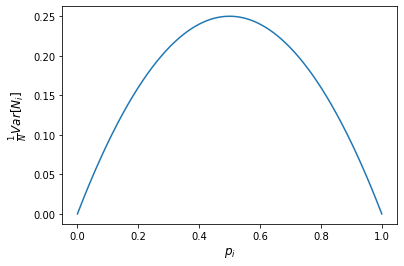
\includegraphics[width=0.3\textwidth]{figures/histogram_variance.png}
    \caption{Plot of normalised variance against bin probability}
    \label{fig:histogram_variance}
\end{figure}


%%%%%%%%%%%%%%%%%%%%%%%%%%
%%%%%%%%%%%%%%%%%%%%%%%%%%

\section{Generating random numbers using functions of other random numbers}

Samples from new distributions can be generated by transforming samples from existing distributions.
The PDF of the new distribution, $p_Y(y)$, can be found using the initial distribution, $p_X(x)$, and
the Jacobian of the transformation, as follows:

\begin{align*}
    p_Y(y) = \sum_{k=1}^K \left. \frac{p_X(x)}{\left|\frac{dy}{dx}\right|} \right|_{x=x_k(y)}
\end{align*}
where $\{x_1(y) \dots x_K(y)\}$ is the set of values for $f^{-1}(y)$.

\subsection{$f(x) = a x + b$}
For $x \sim \mathcal{N}(0, 1)$, let $y = f(x) = a x + b$. Then:
\begin{align*}
    f^{-1}(y) &= \frac{y - b}{a} \\
    \left|\frac{dy}{dx}\right| &= |a| \\
    p_Y(y) &= \frac{1}{|a|} p_X \left( \frac{y - b}{a} \right) \\
    &= \frac{1}{|a|}\times\frac{1}{\sqrt{2\pi}} \exp{\left( -\frac{1}{2} \left( \frac{y-b}{a} \right)^2 \right)}
\end{align*}
Comparing with the equation for a general Gaussian distribution, it is clear that $p_Y(y)$ is a Gaussian distribution
with mean $b$ and variance $a^2$.
The result is compared with a histogram of transformed samples in \autoref{fig:linear_function_of_gaussian}. The close
agreement suggests this hypothesis is correct.

\begin{figure}[h]
    \centering
    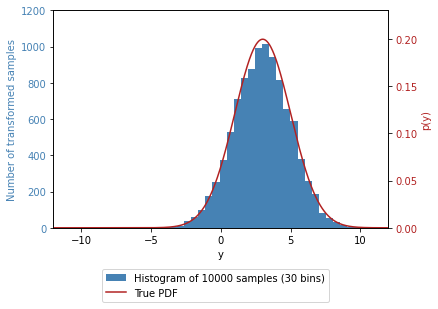
\includegraphics[width=0.6\textwidth]{figures/linear_function_of_gaussian.png}
    \caption{Histogram of linear function ($f(x^{(i)}) = 2x^{(i)} + 3$) of Gaussian samples overlaid with
    calculated PDF}
    \label{fig:linear_function_of_gaussian}
\end{figure}

%%%%%%%%%%%%%%%%%%%%%%%%%%

\subsection{$f(x) = x^2$}
For $x \sim \mathcal{N}(0, 1)$, let $y = f(x) = x ^ 2$. Then:
\begin{align*}
    f^{-1}(y) &= \pm \sqrt{y} \\
    \left|\frac{dy}{dx}\right| &= |2x| \\
    p_Y(y) &= \sum_{i=1}^{2} \frac{1}{|2 \sqrt{y}|} p_X \left( \sqrt{y} \right) \\
    &= \frac{1}{\sqrt{2\pi y}} \exp{\left( -\frac{1}{2} y \right)}
\end{align*}

The result is compared with a histogram of transformed samples in \autoref{fig:quadratic_function_of_gaussian}. The
close agreement suggests this hypothesis is correct.

\begin{figure}[h]
    \centering
    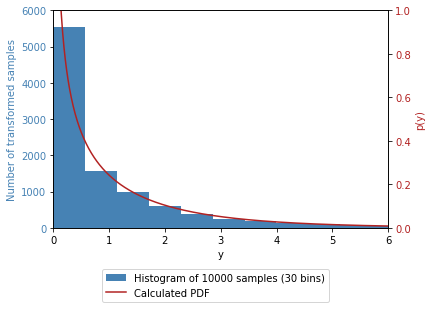
\includegraphics[width=0.6\textwidth]{figures/quadratic_function_of_gaussian.png}
    \caption{Histogram of quadratic function $\left(f(x^{(i)}) = \left(x^{(i)}\right)^2\right)$ of Gaussian samples
    overlaid with calculated PDF}
    \label{fig:quadratic_function_of_gaussian}
\end{figure}

%%%%%%%%%%%%%%%%%%%%%%%%%%

\subsection{$f(x) = \sin(x)$}
For $x \sim \mathcal{U}(0, 2\pi)$, let $y = f(x) = \sin(x)$. Then:
\begin{align*}
    p(x) &= \frac{1}{2\pi} \\
    f^{-1}(y) &= \sin^{-1}(y) \\
    \left|\frac{dy}{dx}\right| &= |\cos(x)| \\
    p_Y(y) &= \sum_{i=1}^{2} \frac{\frac{1}{2\pi}}{\left| \cos\left(\sin^{-1}(y)\right) \right|}
\end{align*}
By drawing a right-angled triangle with hypotenuse of length 1 and a side of length $y$, and applying trigonometry and
Pythagoras' theorem, it can be shown that:
\begin{align*}
    \cos\left(\sin^{-1}(y)\right) = \sqrt{\left(1 -y^2 \right)}
\end{align*}
Hence:
\begin{align*}
    p_Y(y) &= \frac{1}{\pi \sqrt{\left(1- y^2\right)}}
\end{align*}
The result is compared with a histogram of transformed samples in \autoref{fig:sinusoidal_function_of_uniform}. The
close agreement suggests this hypothesis is correct.

\begin{figure}[h]
    \centering
    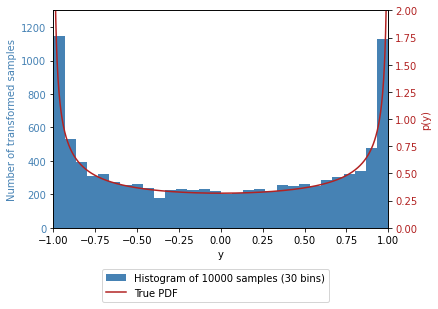
\includegraphics[width=0.6\textwidth]{figures/sinusoidal_function_of_uniform.png}
    \caption{Histogram of sinusoidal function $\left(f(x^{(i)}) = \sin\left(x^{(i)}\right)\right)$ of Uniform samples
    overlaid with calculated PDF}
    \label{fig:sinusoidal_function_of_uniform}
\end{figure}

%%%%%%%%%%%%%%%%%%%%%%%%%%

\subsection{$f(x) = \text{clip}(\sin(x), 0.7)$}
For $x \sim \mathcal{U}(0, 2\pi)$, let:
\begin{align*}
    y = f(x) = \begin{cases}
                   -0.7 & \sin(x) < -0.7 \\
                   \sin(x) & |\sin(x)| < 0.7 \\
                   0.7 & \sin(x) > 0.7
               \end{cases}
\end{align*}
Note that this function differs from the one in the handout by being symmetric, which is a better model of realistic
signal clipping.
This produces a probability density with the following properties:
\begin{itemize}
    \item $|y|$ will never be exceed $0.7$. Hence $p_Y(y)$ will be zero for $|y| > 0.7$.
    \item $f(x)$ collapses all values less than $-0.7$ to $-0.7$, and all values greater than $0.7$ to $0.7$. Hence
          $p_Y(y)$ will have delta functions at $y = 0.7$ and $y = -0.7$, containing all of the probability mass
          from $y > 0.7$ and $y < -0.7$ respectively.
    \item For $|y| < 0.7$, $p_Y(y) = \frac{1}{\pi \sqrt{\left(1- y^2\right)}}$ as before.
\end{itemize}
The area $A$ of each delta function can be calculated using the fact that the PDF must integrate to 1:
\begin{align*}
    A &= \frac{1}{2}\left(1 - \int_{-0.7}^{0.7} \frac{1}{\pi\sqrt{1 - y^2}}\,dy \right) \\
    &= \frac{1}{2} - \frac{1}{\pi} \sin^{-1}(0.7)
\end{align*}
Which gives the PDF as:
\begin{align*}
    p_Y(y) = \begin{cases}
                 A \delta(y + 0.7) & y = -0.7 \\
                 \frac{1}{\pi \sqrt{\left(1- y^2\right)}} & |y| < 0.7 \\
                 A \delta(y - 0.7) & y = 0.7 \\
                 0 & \text{otherwise}
             \end{cases}
\end{align*}
The presence of the delta function in the PDF can also be explained using the Jacobian formula. Consider the derivative
of y:
\begin{align*}
    & \frac{dy}{dx} =
    \begin{cases}
        \cos(x) & 0 < x < \sin^{-1}(0.7) \\
        0 & \sin^{-1}(0.7) < x < \pi - \sin^{-1}(0.7) \\
        \cos(x) & \pi - \sin^{-1}(0.7) < x < \pi + \sin^{-1}(0.7) \\
        0 & \pi + \sin^{-1}(0.7) < x < 2\pi - \sin^{-1}(0.7)
   \end{cases}
\end{align*}
As the Jacobian formula involves dividing by $\frac{dy}{dx}$, $p_Y(y)$ is undefined for the range $|y| > 0.7$, which
indicates the presence of a delta function in the PDF.

The calculated PDF is compared with a histogram of transformed samples in \autoref{fig:sinusoidal_function_of_uniform}.
The close agreement suggests this hypothesis is correct.

\begin{figure}[h]
    \centering
    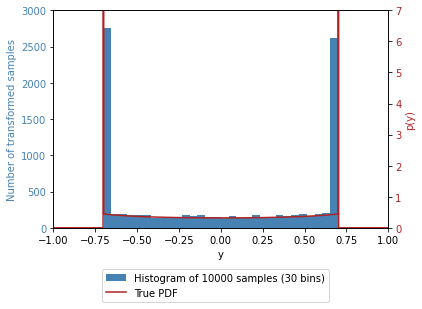
\includegraphics[width=0.6\textwidth]{figures/limited_sinusoidal_function_of_uniform.png}
    \caption{Histogram of limited sinusoidal function $\left(f(x^{(i)}) = \text{clip}\left(\sin\left(x^{(i)}\right), 0.7\right)\right)$
        of Uniform samples overlaid with calculated PDF}
    \label{fig:limited_sinusoidal_function_of_uniform}
\end{figure}

%%%%%%%%%%%%%%%%%%%%%%%%%%
%%%%%%%%%%%%%%%%%%%%%%%%%%

\section{Generating random numbers using the inverse CDF method}

Samples from a distribution with PDF $p_Y(y)$ can sometimes be generated from the uniform distribution
$p_X(x) = \mathcal{U}(x | 0, 1)$ by using the inverse cumulative density function of $Y$
\begin{align*}
    y^{(i)} = F_Y^{-1} \left( x^{(i)} \right)
\end{align*}

\subsection{Exponential distribution}
For the exponential distribution with mean one:
\begin{align*}
    & \text{PDF: } p(y) = \exp(-y), \ y \geq 0 \\
    & \text{CDF: } F(y) = \int_0^y p(y') dy' = 1 - \exp(-y) \\
    & \text{iCDF: } F^{-1}(x) = -\ln(1 - x)
\end{align*}

\autoref{fig:icdf_exponential} shows that samples from the exponential distribution generated using the iCDF follow the
true PDF.

\begin{figure}[h]
    \centering
    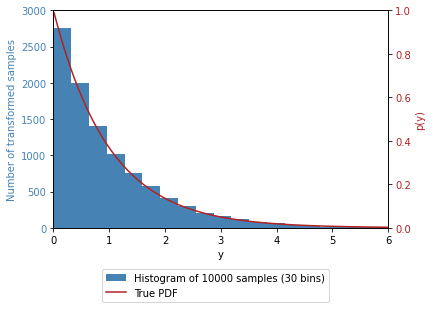
\includegraphics[width=0.6\textwidth]{figures/icdf_exponential.png}
    \caption{Histogram of samples drawn from the uniform distribution and transformed using the iCDF method to follow the
    exponential distribution, overlaid with the true exponential PDF}
    \label{fig:icdf_exponential}
\end{figure}

\subsection{Estimating properties of the exponential distribution}

Properties of the distribution can be estimated using Monte Carlo methods:

\begin{align*}
    \hat{\mu} &= \frac{1}{N} \sum_{i=1}^N y^{(i)} \\
    \hat{\sigma^2} &= \frac{1}{N} \sum_{i=1}^N \left(y^{(i)}\right)^2 - \hat{\mu}^2
\end{align*}

\subsubsection{Properties of Monte Carlo mean estimator}

The Monte Carlo mean estimate $\hat{\mu}$ can be shown to unbiased:

\begin{align*}
    \mathbb{E}[\hat{\mu}] & = \mathbb{E}\left[\frac{1}{N} \sum_{i=1}^N y^{(i)}\right] \\
    &= \frac{1}{N} \sum_{i=1}^N \mathbb{E}\left[y^{(i)}\right] = \frac{1}{N} \sum_{i=1}^N \mu \\
    &= \frac{N\mu}{N} = \mu
\end{align*}

To derive the variance of the Monte Carlo mean estimator, consider the variance of the sum of random variables $X$ and
$Y$:

\begin{align*}
    Var[X+Y]
    &= \mathbb{E}\left[(X + Y - \mu_X - \mu_Y)^2\right] \\
    &= \mathbb{E}\left[((X - \mu_X) + (Y - \mu_Y))^2\right] \\
    &= \mathbb{E}\left[(X-\mu_X)^2\right]] + \mathbb{E}\left[(Y-\mu_Y)^2\right] + 2\mathbb{E}\left[(X-\mu_X)(Y-\mu_Y)\right]
\end{align*}

Using the fact that $X$ and $Y$ are independent gives $\mathbb{E}\left[(X-\mu_X)(Y-\mu_Y)\right] = 0$, hence:

\begin{align*}
    Var[X+Y] & = Var[X] + Var[Y]
\end{align*}

When multiplying a random variable by a scalar, the variance is multiplied by the square of the scalar:

\begin{align*}
    Var[kX]
    &= \mathbb{E}\left[(kX)^2\right] - \mathbb{E}[kX]^2 \\
    &= k^2 \mathbb{E}\left[X^2\right] - k^2\mathbb{E}[X]^2 \\
    &= k^2 Var[kX]
\end{align*}

Treating the samples $y^{(i)}$ as independent random variables and combining the above properties gives:

\begin{align*}
    Var\left[ \frac{1}{N}\sum_{i=1}^N y^{(i)} \right] &= \frac{1}{N^2} \sum_{i=1}^N Var\left[y^{(i)}\right] = \frac{\sigma}{N}
\end{align*}

The convergence of the Monte Carlo estimators for the mean and variance is shown in \autoref{fig:monte_carlo_convergence}.
It is apparent that the mean estimator does indeed converge proportional to $\frac{1}{N}$
(see \autoref{fig:monte_carlo_mean_best_fit}).

\begin{figure}[h]
    \centering
    \begin{subfigure}[b]{0.3\textwidth}
        \centering
        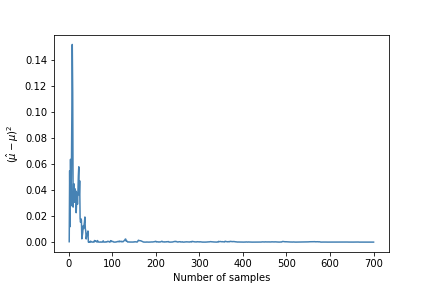
\includegraphics[width=\textwidth]{figures/monte_carlo_mean.png}
        \caption{$\hat{\mu} = \frac{1}{N} \sum_{i=1}^{N} y^{(i)}$}
        \label{fig:monte_carlo_mean}
    \end{subfigure}
    \hfill
    \begin{subfigure}[b]{0.3\textwidth}
        \centering
        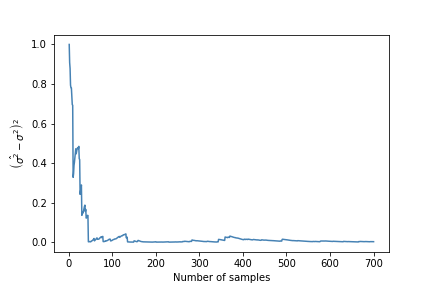
\includegraphics[width=\textwidth]{figures/monte_carlo_variance.png}
        \caption{$\hat{\sigma^2} = \frac{1}{N} \sum_{i=1}^N \left(y^{(i)}\right)^2 - \hat{\mu}^2$}
        \label{fig:monte_carlo_variance}
    \end{subfigure}
    \hfill
    \begin{subfigure}[b]{0.3\textwidth}
        \centering
        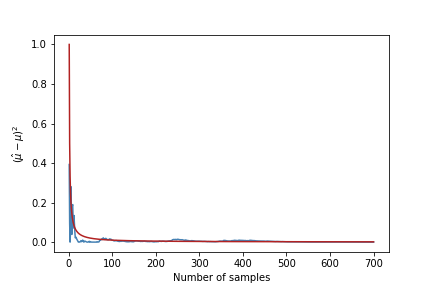
\includegraphics[width=\textwidth]{figures/monte_carlo_mean_best_fit.png}
        \caption{$\hat{\mu}$ with $\frac{1}{N}$ overlay}
        \label{fig:monte_carlo_mean_best_fit}
    \end{subfigure}
    \caption{Behaviour of Monte Carlo estimators for increasing number of samples}
    \label{fig:monte_carlo_convergence}
\end{figure}

\subsubsection{Application to the exponential distribution}
The exponential distribution $p(y) = \exp(-y), \ y \geq 0$ has $\mu = 1$ and $\sigma^2 = 1$.
Applying Monte Carlo estimation to 10000 samples gives $\hat{\mu} = 1.0035$ and $\hat{\sigma^2} = 1.0128$, which are
close to the true values.


%%%%%%%%%%%%%%%%%%%%%%%%%%
%%%%%%%%%%%%%%%%%%%%%%%%%%

\section{Generating random numbers using a scaled mixture of Gaussians}

Samples from more complex distributions can sometimes be generated using samples from Gaussian distributions
where the variance of the Gaussian is set by another distribution, $p(u)$:
\begin{align*}
    p(x) = \int_0^{\infty} \mathcal{N}(x | 0, u) p(u) du
\end{align*}

\subsection{Setting the variance with the Exponential distribution}

Samples $u^{(i)}$ can be generated from the distribution with the following PDF:
\begin{align*}
    p(u) = \frac{\alpha^2}{2} \exp\left(-\frac{\alpha^2}{2} u \right)
\end{align*}
This distribution has:
\begin{align*}
    & \text{CDF: } F(u) = \int_0^u p(u') du' = 1 - \exp\left(-\frac{\alpha^2}{2} u\right) \\
    & \text{iCDF: } F^{-1}(v) = -\frac{2}{\alpha^2} \ln(1 - v)
\end{align*}
Hence samples $u^{(i)}$ can be generated from Uniformly distributed random samples $v^{(i)}$ using the iCDF method.
The samples $u^{(i)}$ are then used to set the variance of the random variable X:
\begin{align}\label{eq:exponential_sampled_gaussian}
    p(x) = \int_{0}^{\infty} \mathcal{N}(x\,|0, u) \frac{\alpha^2}{2} \exp\left(-\frac{\alpha^2}{2} u \right) du
\end{align}
The limit of the integral is from zero to infinity because the standard deviation must be positive.
A histogram of samples of $x^{(i)}$ is plotted in \autoref{fig:exponential_sampled_gaussian} for different values of
$\alpha$. It appears that $\alpha$ sets the standard deviation of the distribution.

\begin{figure}[h]
    \centering
    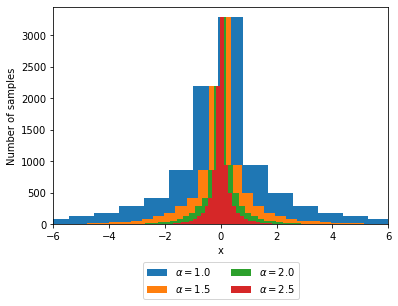
\includegraphics[width=0.6\textwidth]{figures/exponential_sampled_gaussian.png}
    \caption{100-bin histogram of samples drawn from the distribution in \autoref{eq:exponential_sampled_gaussian} for
    different values of $\alpha$}
    \label{fig:exponential_sampled_gaussian}
\end{figure}

The kernel method was applied to the data, and the smoothed density was plotted on linear and log axes at different
scales (\autoref{fig:nonstandard_distribution_kernel_smoothed}\footnote{Note that
\autoref{fig:nonstandard_distribution_ksdensity_log_far} provides little useful information for the tail behaviour of
the distribution, as there are very few samples for the extreme tails, so the plot is dominated by the
behaviour of the kernel.}).
From the shape of the distribution, it appears to be a sharper version of a Gaussian distribution, with significantly
higher probability density in the centre and tails that last for longer.
From \autoref{fig:nonstandard_distribution_ksdensity_log_wide} it appears that the distribution may follow some
exponential relationship, as the tails appear approximately linear on the logarithmic plot.
It can also be observed that the distribution is symmetric about zero.
Combining these properties suggests that the PDF might be:
\begin{align*}
    p(x) \sim \exp(-|x|)
\end{align*}


\begin{figure}[h]
    \centering
    \begin{subfigure}[b]{0.3\textwidth}
        \centering
        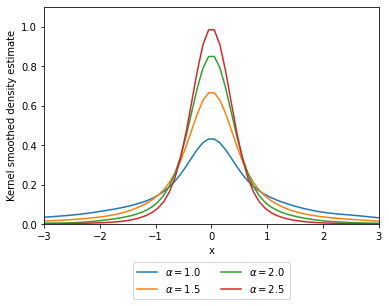
\includegraphics[width=\textwidth]{figures/nonstandard_distribution_ksdensity.png}
        \caption{Linear scale}
        \label{fig:nonstandard_distribution_kernel_smoothed_linear}
    \end{subfigure}
    \hfill
    \begin{subfigure}[b]{0.3\textwidth}
        \centering
        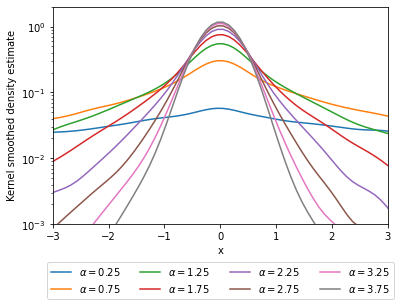
\includegraphics[width=\textwidth]{figures/nonstandard_distribution_ksdensity_log_close.png}
        \caption{$10^{-3} < \log(p(x)) < 1$}
        \label{fig:nonstandard_distribution_ksdensity_log_close}
    \end{subfigure}
    \hfill
    \begin{subfigure}[b]{0.3\textwidth}
        \centering
        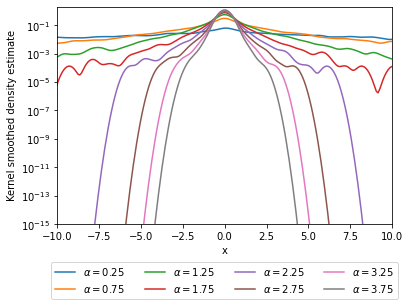
\includegraphics[width=\textwidth]{figures/nonstandard_distribution_ksdensity_log_far.png}
        \caption{$10^{-15} < \log(p(x)) < 1$}
        \label{fig:nonstandard_distribution_ksdensity_log_far}
    \end{subfigure}
    \caption{Kernel smoothed probability density estimates for the example distribution}
    \label{fig:nonstandard_distribution_kernel_smoothed}
\end{figure}

%%%%%%%%%%%%%%%%%%%%%%%%%%

\subsection{Setting the variance with the Gamma distribution}
\subsubsection{PDF of $U=\frac{1}{V}$}
The probability density function of the random variable $U$ can be calculated by applying the Jacobian method:
\begin{align*}
     p(v) &= \mathcal{G}(v | \theta, \theta^{-1}) \\
    &= \frac{1}{\theta^{-\theta} \Gamma (\theta)} v^{\theta - 1} e^{-v \theta} \\
    \left| \frac{du}{dv} \right| &= \left| -v^{-2} \right| = v^{-2} \\
    f^{-1} (u) &= u^{-1}
\end{align*}
Hence:
\begin{align*}
    p(u) &= \left. \frac{p(v)}{v^{-2}} \right|_{v=u^{-1}} \\
    &= \frac{\theta^{\theta}}{u^2 \Gamma(\theta)} u^{1-\theta} e^{-\frac{\theta}{u}}
\end{align*}
\begin{align}\label{eq:pdf_of_u}
    p(u) &= \frac{\theta^{\theta}}{\Gamma(\theta)} u^{-1-\theta} e^{-\frac{\theta}{u}}
\end{align}

\subsubsection{PDF of $X \sim \mathcal{N}(0, u)$}
The PDF of $X \sim \mathcal{N}(0, u)$, where $p(u)$ is taken from \autoref{eq:pdf_of_u}, can be obtained by
marginalisation:
\begin{align*}
    p(x) &= \int_0^\infty \mathcal{N}(x | 0, u) p(u) du \\
    &= \int_0^\infty \frac{1}{\sqrt{2\pi}} u^{-\frac{1}{2}} e^{-\frac{1}{2} x^2 u^{-1}}
    \frac{\theta^{\theta}}{\Gamma(\theta)} u^{-1-\theta} e^{-\theta u^{-1}} du \\
    &= \frac{\theta^{\theta}}{\sqrt{2\pi} \Gamma(\theta)}
    \int_0^\infty \left( u^{-1} \right) ^ {\frac{3}{2} + \theta} e^{-\left( \theta + \frac{1}{2} x^2 \right) u^{-1}} du
\end{align*}
Performing a change of variable on $u$ by setting $u = v^{-1}$, and using the fact that $\frac{du}{dv} = -v^{-2}$,
gives:
\begin{align*}
    p(x) &= - \frac{\theta^{\theta}}{\sqrt{2\pi} \Gamma(\theta)}
    \int_{-\infty}^0 v ^ {\frac{3}{2} + \theta} e^{-\left( \theta + \frac{1}{2} x^2 \right) v} v^{-2} dv
\end{align*}
\begin{align}\label{eq:p(x)_integral}
    p(x) = \frac{\theta^{\theta}}{\sqrt{2\pi} \Gamma(\theta)}
    \int_0^\infty v ^ {-\frac{1}{2} + \theta} e^{-\left( \theta + \frac{1}{2} x^2 \right) v} dv
\end{align}
From the definition of the Gamma distribution, we know that:
\begin{align*}
    \int_0^\infty v ^ {a - 1} e^{-\frac{v}{b}} dv = b^a \Gamma(a)
\end{align*}
Which is the integral from \autoref{eq:p(x)_integral} with
\begin{align*}
    a &= \theta + \frac{1}{2} \\
    b &= \left(\theta + \frac{1}{2} x^2 \right) ^ {-1}
\end{align*}
Hence \autoref{eq:p(x)_integral} solves to become:
\begin{align}
    p(x) = \frac{\theta^{\theta} \Gamma\left(\theta + \frac{1}{2} \right)}{\sqrt{2\pi} \Gamma(\theta)}
    \left( \theta + \frac{1}{2}x^2 \right)^{-\theta - \frac{1}{2}}
\end{align}
When $|x|$ is large,

%%%%%%%%%%%%%%%%%%%%%%%%%%

\newpage
%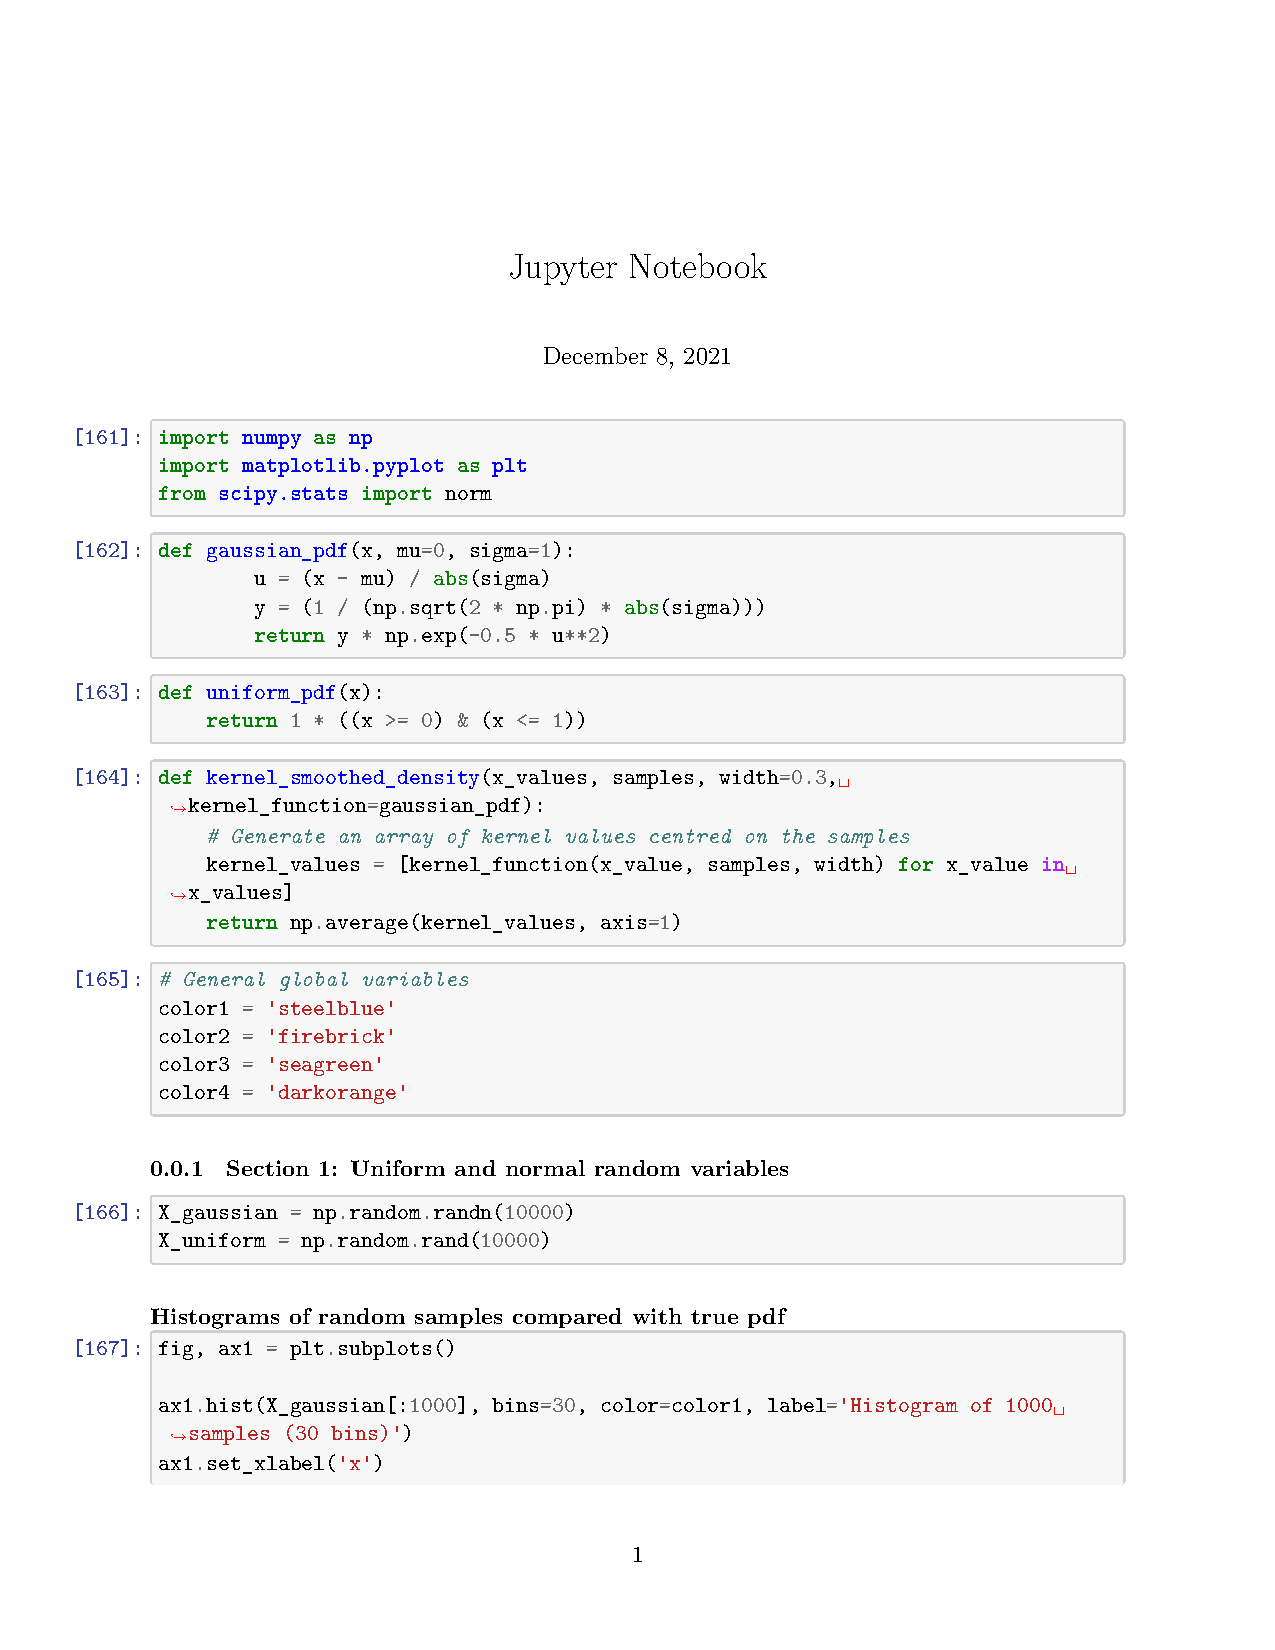
\includepdf[pages=-]{out/Jupyter Notebook.pdf}

\end{document}